\documentclass[10pt, titlepage, oneside, a4paper]{article}
\usepackage[T1]{fontenc}
\usepackage[utf8]{inputenc}
\usepackage[swedish]{babel}
\usepackage{amssymb, graphicx, fancyhdr}
\usepackage{hyperref}
\usepackage{pgf, tikz}
\usepackage{pgfplots}
\usepackage{listings}
\usepackage{color}
\usepackage{amsmath}
\usepackage{mathtools}
\usepackage{float}
\addtolength{\textheight}{20mm}
\addtolength{\voffset}{-5mm}
\renewcommand{\sectionmark}[1]{\markleft{#1}}

\newcommand{\Section}[1]{\section{#1}\vspace{-8pt}}
\newcommand{\Subsection}[1]{\vspace{-4pt}\subsection{#1}\vspace{-8pt}}
\newcommand{\Subsubsection}[1]{\vspace{-4pt}\subsubsection{#1}\vspace{-8pt}}


\def\typeofdoc{Laborationsrapport}
\def\course{F0004T}
\def\pretitle{Laboration 1}
\def\title{Svängningstid av svängande svängningar}
\def\username{magbjr-3}
\def\domain{@student.ltu.se}
\def\email{\username{}@student.ltu.se}
\def\group{Grupp 10}
\def\graders{Magnus Frediksson}
\def\university{Luleå Tekniska Universitet}


\def\fullpath{\raisebox{1pt}{$\scriptstyle \sim$}\username/\path}


\begin{document}
	\begin{titlepage}
		\thispagestyle{empty}
		\begin{large}
			\begin{tabular}{@{}p{\textwidth}@{}}
				\textbf{\university\hfill\today}\\
				\textbf{\typeofdoc} \\
			\end{tabular}
		\end{large}
		\vspace{10mm}
		\begin{center}
			\LARGE{\pretitle} \\
			\huge{\textbf{\course}}\\
			\vspace{10mm}
			\LARGE{\title}\\
			\vspace{15mm}
			\begin{large}
				\begin{tabular}{l|ll}
                    \textbf{\group} & \textbf{Namn} & \textbf{E-mail}\\
                    \hline
                    & \texttt{Anton Eriksson}   & \texttt{eriano-4\domain}       \\
                    & \texttt{Eric Öhman}   & \texttt{erihma-3\domain}       \\
                    & \texttt{Magnus Björk}   & \texttt{magbjr-3\domain}       \\
				\end{tabular}
			\end{large}
			\vfill
			\large{\textbf{Handledare}}\\
			\mbox{\large{\graders}}
		\end{center}
	\end{titlepage}


	\lfoot{\footnotesize{\group}}
	\rfoot{\footnotesize{\today}}
	\lhead{\sc\footnotesize\title}
	\rhead{\nouppercase{\sc\footnotesize\leftmark}}
	\pagestyle{fancy}
	\renewcommand{\headrulewidth}{0.2pt}
	\renewcommand{\footrulewidth}{0.2pt}

	\pagenumbering{roman}
    \begin{abstract}
    \end{abstract}
    
    \tableofcontents
	
	\newpage
	\pagenumbering{arabic}

	\setlength{\parindent}{10pt}
	\setlength{\parskip}{10pt}
    
	\section{Inledning}
    Vi har fått i uppgift att ta fram ett uttryck för svängningstiden T hos en balk som befinner sig i svängning.\\\\Balkens ena sida sitter fastspänd i ett skruvstäd, dess andra sida befinner sig fritt i luften. Trycker man ned den fria sidan kommer balken att börja svänga upp och ned. Det är den tid det tar för balken att svänga från dess lägsta till högsta läge som vi beskriver i denna rapport. 
	\section{Metod}
    För att strukturera arbetet gjordes en planering av laborationen. Detta görs enligt en standardiserad metod som är vanlig i projekt som detta där samband ska tas fram.
    \begin{enumerate}
        \item Deifiniera Problemet.
        \item Vad påverkar?
        \item Planera mätningar.
        \item Resultat Tabell.
        \item Rita Figurer.
        \item Analysera (Linjärisera).
        \item Dimensionsanalys.
    \end{enumerate}

Materialen som användes i laborationen: Ställning för balkar, fotocell, dosa för avläsning av fotocellens mätningar, balkar i fyra olika material samt olika dimensioner, måttband.

 Fyra olika tester genomfördes för att kunna ta fram sambandet mellan period tiden och ändringen i längd, tjocklek, bredd och material.
Mätningarna utfördes genom att man fäste balken som skulle testas i ställningen. Balken fästes bara i ena änden medans den andra änden var fri och kunde röra sig i vertikalled. I den fria änden placerades fotocellen för att kunna mäta balkens svängningstid. Fotocellen placerades så nära balkens ände som möjligt för att   I första testet användes endast en stålbalk. Det enda som ändrades i detta test var längden på balken.

    \newpage
    \section{Analys}
    
        \subsection{Variabellista}
        \begin{table}[h]
            \begin{tabular}{lccl}
            \hline
            \textbf{Storhet} & \textbf{Symbol} & \textbf{Enhet} & \textbf{Grunddimension} \\ \hline
            Pendeltid    & T    & s     & T          \\ 
            Balklängd    & l    & m     & L          \\ 
            Balktjocklek & d    & m     & L          \\ 
            Balkbredd    & b    & m     & L          \\ 
            Densitet     & $\rho$    & $kg/m^3$ & $M\cdot L^{-3}$     \\ 
            E-modul      & E      & \footnotesize $kg/ms^2$    &$M\cdot L^{-1}\cdot T^{-2}$                \\ \hline
            \end{tabular}
        \end{table} 
        
	\section{Resultat}
        \subsection{Hur påverkar balkens längd svängningstiden?}
        \begin{table}[H]
            \caption{Undersökning av längd.}
            \begin{center}
                \begin{tabular}{cc}
                    \hline
                    Tid (s) & Längd (m) \\
                    \hline
                    0.362 & 1.200 \\
                    0.305 & 1.100 \\
                    0.254 & 1.000 \\
                    0.207 & 0.900 \\
                    0.164 & 0.800 \\
                    0.145 & 0.750 \\
                    0.094 & 0.600 \\
                    0.066 & 0.500 \\
                    0.083 & 0.400 \\
                \end{tabular}
            \end{center}
        \end{table}
        Vid undersökning av hur balklängden påverkar svängningstid antogs funktionen:

        \begin{equation}
        T=a\:l^b
        \end{equation}

        Där $T$ är pendeltiden, $a$ är en okänd konstant, $l$ är balklängden och $b$ är ytterliggare en okänd konstant. För att ta reda på de okända konstanterna så lineariserade vi mätdatat och gjorde en ny plot. Efter logaritmeringen av mätvärdena liknar trendlinjen en linjär funktion. Genom att lösa ekvationen för den räta trendlinjen kan vi lösa ut konstanterna $a$ och $b$.\\

        Räta linjens ekvation:

        \begin{equation}
        y=kx+m
        \end{equation}
        \begin{center}
        $y=ln\:T$, $k = b$, $x = ln\:l$ och $m = ln\:a$ \\
        \end{center}

        \vspace{10pt}
        Trendlinjens ekvation (\ref{trendeq1}) och lösning för konstanterna a och b:

        \begin{equation}\label{trendeq1}
        y=1,9495\,x-1,37
        \end{equation}

        \begin{center}
        $ln\:a=m=-1,37$ \\
        $e^{ln\:a} = e^{-1,37}=0,254$ \\
        $a=0,254$ \\
        \vspace{10pt}
        $b=1,9495$
        \end{center}

        \vspace{10pt}
        Pendeltiden som funktion av balkens längd blir således:
        \begin{equation}\label{lengtheq1}
        T=0,254\ l^{1,9495}
        \end{equation}
        
        \begin{figure}[H]
            \centering
            \includegraphics[scale=.5]{../png/length.png}
            \caption{Svängningstid beroende på längd.}
            \label{length}
        \end{figure}

        \subsection{Hur påverkar balkens tjocklek svängningstiden?}
        \begin{table}[H]
            \caption{Undersökning av tjocklek.}
            \begin{center}
                \begin{tabular}{cccc}
                    \hline
                    Tid (s) &Tjocklek (m)\\
                    \hline
                    0.421 & 0.003\\
                    0.254 & 0.005\\
                    0.215 & 0.006\\
                    0.162 & 0.008\\
                \end{tabular}
            \end{center}
        \end{table}  

Vid undersökning av hur balktjockleken påverkar pendeltiden antogs funktionen:

\begin{equation}
T=c\:h^d
\end{equation}
\begin{center}
Där $T$ är pendeltiden, $c$ är en okänd konstant, $h$ är balktjockleken och $d$ är ytterliggare en okänd konstant. Även denna gång lineariserade vi och undersökte den räta trendlinjens ekvation för att hitta konstanterna $c$ och $d$.\\
\end{center}

\vspace{10pt}
Trendlinjens ekvation (\ref{trendeq2}) och lösning för konstanterna $c$ och $d$:
\begin{equation}\label{trendeq2}
y=-0,972\ x - 6,515
\end{equation}

\begin{center}
$ln\:c=m=-6,515$ \\
$e^{ln\:c} = e^{-6,515}=0,0014$ \\
$c=0,0014$ \\
\vspace{10pt}
$d=-0,972$
\end{center}

\vspace{10pt}
Pendeltiden som funktion av balkens tjocklek blir således:
\begin{equation}\label{thicknesseq1}
T=0,0014\ h^{-0,972}
\end{equation}
        

        \subsection{Hur påverkar balkens bredd svängningstiden?}
        \begin{table}[H]
            \caption{Undersökning av bredd.}
            \begin{center}
                \begin{tabular}{cc}
                    \hline
                    Tid (s) & Tjocklek (m)\\
                    \hline
                    0.255 & 0.020\\
                    0.259 & 0.025\\
                    0.250 & 0.030\\
                    0.259 & 0.040\\
                \end{tabular}
            \end{center}
            Balkens bredd påverkar ej svängningstiden.
        \end{table}
        \subsection{Dimensionsanalys}

Tidigare har vi tagit fram två olika funktioner, den ena funktionen beskriver hur längden påverkar pendeltiden (\ref{lengtheq1}) och den andra funktionen beskriver hur tjockleken påverkar pendeltiden(\ref{thicknesseq1}). Målet med dimensionanalysen är att ta fram en funktion som innehåller de variablar som påverkar pendeltiden. $E$ = E-modul, vilket är ett mått på ett materials elasticitet. Vi tog även med densitet $\rho$ i dimensionsanalysen. Exponenterna till balkens längd och tjocklek som vi tidigare löste ut genom linearisering avrundades för att underlätta dimensionsanalysen:

\begin{center}
Balklängden $l^{1,9495} \approx l^2$ och balktjockleken $h^{-0,972} \approx h^{-1}$\\
\vspace{18pt}
Uppställning av ekvation för dimensionsanalys:
\end{center}


\begin{equation}\label{dimeq1}
T= l^2 h^{-1} E^\alpha \rho ^\beta C
\end{equation}

\begin{description}
 \item $T$ = Pendeltid i sekunder
 \item $l$ = Balklängd i meter
 \item $h$ = Balktjocklek i meter
 \item $E$ = Elasticitets-modul
 \item $\rho$ = Densitet
 \item $C$ = Okänd konstant
\end{description}

\vspace{10pt}



Grunddimensioner i VL och HL:
\begin{equation}
T^1M^0L^0= L^2  L^{-1} (M^1L^{-1}T^{-2})^\alpha   (M^1L^{-3})^\beta  C
\end{equation}


Ger ekvationssystemet:
\begin{equation}
\begin{cases}
   1 = -2\alpha \\
   0 = \alpha + \beta \\
   0 = 1 - \alpha - 3\beta
\end{cases}
\end{equation}


Lösningarna:
\begin{equation}
\begin{cases}
   \alpha = -\frac{1}{2}\\
   \beta = \frac{1}{2}
\end{cases}
\end{equation}


$\alpha$ och $\beta$ insättes i ekvation (\ref{dimeq1})
\begin{equation}
T=h^{-1}   l^2  E^{-\frac{1}{2}}  \rho ^\frac{1}{2}  C
\end{equation}

C kan nu lösas ut eftersom övriga variabler är kända:
\begin{equation}
C=\frac{T}{h^{-1}   l^2  E^{-\frac{1}{2}}  \rho ^\frac{1}{2}}
\end{equation}

Kända värden insättes för att lösa C:\\
Tid $T=0,254$ s, längd $l=1,0$ m, tjocklek $b=0,005$ m, E-modul stål $E=200\cdot 10^9$ $kg/ms^2$, uppmätt densitet $7761$ $kg/m^3$

\begin{equation}
C=\frac{0,254}{0,005^{-1}   1,0^2  (200\cdot 10^9)^{-\frac{1}{2}}  7761^\frac{1}{2}} = 6,4470 \approx 6,45
\end{equation}

\vspace{10pt}
SLUTGILTIGA EKVATIONEN YEEEAAAHH:
\begin{equation}
%T = 6,45\cdot \frac{l^2\sqrt\rho}{h\sqrt{E}}
T = 6,45\ \frac{l^2\sqrt\frac{\rho}{E}}{h}
\end{equation}

        
            
                    
    \begin{figure}[H]
        \centering
        \includegraphics[scale=.5]{../png/height.png}
        \caption{Svängningstid beroende på tjocklek.}
        \label{height}
    \end{figure}
    \begin{figure}[H]
        \centering
        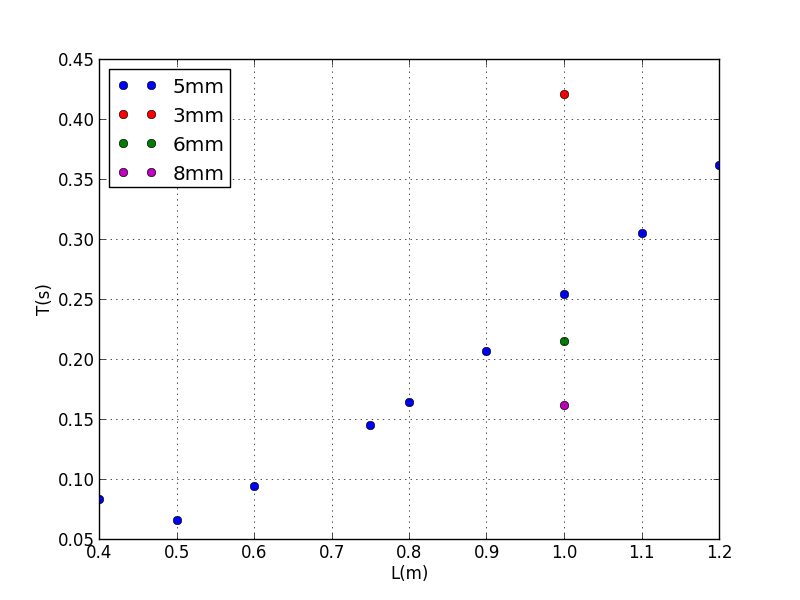
\includegraphics[scale=.5]{../png/plot.png}
        \caption{Svängningstid beroende på material.}
        \label{material}
    \end{figure}
    \begin{figure}[H]
        \centering
        \includegraphics[scale=.5]{../png/ln_t_ln_l.png}
        \caption{linearisering}
        \label{linearisering}
    \end{figure}



    \section{Diskussion}



\end{document}

